\section{Chapter 12. Solids}

\secttoc

{
\footnotesize
\begin{multicols}{3}
    \begin{compactenum}
    \item classify solids based on bonding/IMFs
    \item differences between crystalline and amorphous solids
        (crystal lattice, unit cells, etc)
    \item why are there a limited number of lattices? 5 2D and 7 3D
        primitive lattices
    \item characteristics/properties of metals
    \item empirical formula and density of ionic/metallic solid given a unit cell.\
        estimate length of a cubic unit cell from radii of atoms present
    \item homogeneous/heterogeneous alloys
    \item electron-sea model of metallic bonding
    \item MO model of metallic bonding to generate electronic band structure
        of metals, qualitatively predict MP \& BP, hardness
    \item predict structures of ionic solids given radii and empirical formula
    \item MP \& BP in terms of IMF and crystalline forces
    \item valence/conduction bands. band gap, holes, semiconductor and insulator
    \item account for relative band gap energies of semiconductors through periodic trends
    \item n-type and p-type doping to control conductivity
    \item plastic, thermoplastic, thermosetting plastic, elastomer, copolymers,
        and cross-linking
    \item polymers formed from monomers, what features allow this?
    \item polymer chain interactions impact physical properties
    \item properties of semicond. and metals change with nanometer crystals
    \item structure/properties of fullerenes, carbon nanotubes and graphene
    \end{compactenum}
\end{multicols}
}

\begin{mdframed}
    \subsection{Classification}
    \begin{multicols}{3}
\begin{compactdesc}
    \item[Types of kinetic energy] translational, rotational, vibrational.
        \item[solids] lowest energy phase, mostly vibrational energy
        Atoms packed tight. It is surfaces of solids that react.
        \item[metallic solids] held together by delocalized sea of valence $e^-$
        \item[ionic solids] mutual attraction between anions/cations
        \item[covalent-network solids] extended network of covalent bonds
        \item[molecular solids] weak IMFs
        \item[polymers] long chains of atoms, covalent
        \item[nanomaterials] individual crystals are 1-100nm.
    \end{compactdesc}
\end{multicols}
\end{mdframed}


\begin{mdframed}
    \subsection{Structures}

    \begin{multicols}{3}
\begin{compactdesc}
        \item[crystalline solids] regularly repeating pattern, usually flat
            faces, specific angles
        \item[amorphous solids] no long-range order
        \item[unit cell] smallest repeating unit
        \item[crystal lattice] geometrical pattern of points where unit cells go.
            \emph{N-dimensional} lattices
            can be defined with \emph{n} vectors
        \item[motif,]group of atoms, associated with each \emph{lattice point}
        \item[primitives] 5 2D lattices, 7 3D lattices
        \item[square  ] $a = b, \gamma = 90$
        \item[rect    ] $a \neq b, \gamma = 90$
        \item[hex     ] $a = b, \gamma = 120$
        \item[rhombic ] $a = b$
        \item[oblique ] $a \neq b$
        \item[cubic] $a = b = c, \alpha = \beta = \gamma = 90$
        \item[tetra] $a = b \neq c, \alpha = \beta = \gamma = 90$
        \item[hexa] $a = b \neq c, \alpha = \beta = 90, \gamma = 120$
        \item[rhombohedral] $a = b \neq c, \alpha = \beta = \gamma \neq 90$
        \item[orthorhombic] $a \neq b \neq c, \alpha = \beta = \gamma = 90$
        \item[monoclinic] $a \neq b \neq c, \alpha = \beta = 90, \gamma \neq 90$
        \item[triclinic] $a \neq b \neq c, \alpha \neq \beta \neq \gamma$
        \item[body-centered cubic] additional point at center of such a cell
        \item[face-centered] additional points at the faces of a cell
    \end{compactdesc}
\end{multicols}
\end{mdframed}

\begin{mdframed}
    \subsection{Metallic solids}

    \begin{multicols}{3}
\begin{compactdesc}

    \item[Metallic solids] good conductors of electricity and heat, malleable (sheets), ductile (wires)
    \item[Structure] usually simple, just need one atom on each
        lattice point.
    \item[Primitive] 1 atom per unit cell. \textbf{Body-centered} 2 atoms per.
        \textbf{Face-centered} 4 atoms per.

    \item[Tight packing] is favorable if $e^-$ are shared.
        \textbf{Hexagonal close packing} hcp, \textbf{Cubic} ccp.
    \item[Coordination number] 12 for hcp and ccp. In both,
        each sphere has 12 equidistant neighbors. Any immediate neighbors.

    \item[Alloy] material that contains more than one element and behaves like
        a metal.
    \item[Substitutional alloy] two metallic components have similar radii and
        bonding characteristics. Less typical if radii differ $>15\%$.
    \item[Interstitial alloy] solute atoms must have smaller bonding radii
        than solvent. Extra bonds mean stronger/harder/less ductile.
    \item[Heterogeneous alloy] components are not dispersed uniformly.
        Properties depend on both composition and the manner in which the solid
        was formed from molten mixture (ex: cooled fast/slow?).
    \item[Inter-metallic compounds] not mixtures. Definite properties.

\end{compactdesc}
\end{multicols}
\end{mdframed}



\begin{mdframed}
\subsection{Metallic bonding}

\begin{multicols}{2}
\begin{compactdesc}
    \item[Electron-sea model] metal = array of metal cations in a sea of
        valence electrons. Electrons migrate to positive end. Also, their
        motion facilitates transfer of kinetic energy (heat).
        Not enough $e^-$ on each atom, must share!
    \item[Molecular-orbit model, Band Structure]
        Orbitals shared by entire metal. Fills low \ce{->} high.
        Bands are per-molecule in nonmetals. 3d band, 4s, 4d bands \dots
    \item[Conduction band] easy to remove $e^-$ from here, the top.
    \item[Valence band] $e^-$ stick to here, closest to nucleus.
    \item[Stronger bonds] mean higher boiling/melting points, heats of fusion,
        hardness, and so forth.
    \item[Group 6B] middle, highest strength. More does not always mean more
        strength, repulsion in antibonding MOs can ruin it. Recall bond order
        $\frac{1}{2}$ (bonding $-$ antibonding $e^-$)
\end{compactdesc}
\end{multicols}

\begin{figure}[H]
    \centering
    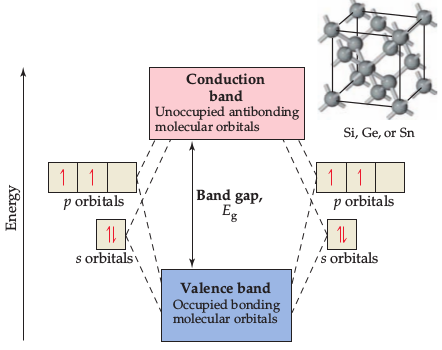
\includegraphics[width=0.5\textwidth]{band_gap.png}
\end{figure}

\end{mdframed}



\begin{mdframed}
\subsection{Complex}

\begin{multicols}{2}
\begin{compactdesc}
\item[Color] caused by $e^{-}$ shuffling about the d-orbital. \ce{TiO2} has
    no electrons in the d-orbital and is colorless.
\end{compactdesc}
\end{multicols}
\end{mdframed}




\begin{mdframed}
    \subsection{Ionic solids}

    \begin{multicols}{3}
\begin{compactdesc}
    \item[Ionic solids] electrostatic attraction between cations and anions.
        Interactions increase as charges of ions increases (lattice energy++).
    \item[Structures] cations are usually much smaller than anions.
    \item[Coordination number] smaller than metals.
        Close packing is prohibited by repulsive forces.
    \item[Formula from structure]
        $\frac
            {\text{Cations per formula unit}}
            {\text{anions per formula unit}}
        $  is equal to
        $ \frac
            {\text{anion coord number}}
            {\text{cation coord number}} $
    \item[No conduction] as solids! Molten salt can conduct.
    \end{compactdesc}
\end{multicols}
\end{mdframed}



\begin{mdframed}
\begin{multicols}{3}

    \subsection{Molecular solids}

\begin{compactdesc}
    \item[Molecular solids] atoms/neutral molecules held by dipole-dipole,
        dispersion, and/or hydrogen bonds.
    \item[Weak bonds] low BP, MP (below 200 Celsius), soft.
        More symmetry means tighter packing, stronger bonds.
\end{compactdesc}

    \subsection{Covalent-network solids}

\begin{compactdesc}
    \item[Strong bonds] covalent bonds beat IMFs. Diamond, quartz.
\end{compactdesc}

    \subsection{Semiconductors}

\begin{compactdesc}
    \item[Semiconductors] harder for $e^-$ to move between levels because of a
        ``band gap'' separating valence/conduction bands.
        Typically group 4 (C, Si, Ge, Sn). Band gap + +, conduction - -
    \item[large band gap] no conduction!
\end{compactdesc}


\end{multicols}
\end{mdframed}



\begin{mdframed}
    \subsection{Polymers}

\begin{multicols}{3}
\begin{compactdesc}
\item[Polymers] chains or branched structures composed of monomers.
\item[Addition Polymerization] two monomers added to each other, double bond
    between is elimintated.
\item[Condensation Polymerization] condensing two monomers together, getting
    rid of intermediate small molecule once they are linked.
\item[Chain inititaion] a free radical initiator possesing an unstable
    unpaired electron attacks a monomer unit to cause it to expose another
    unstable $e^{-}$.
\item[Chain propogation] this unit attacks other monomers, forming an ever
    growing chain.
\item[Polymer crosslinks] produce harder substances with less flexibility.
\item[Commercial example] polyethylene chains contain between $10^3$ and
    $10^5$ \ce{CH2} units.
\end{compactdesc}
\end{multicols}
\end{mdframed}



% \begin{mdframed}
%     \subsection{Nanomaterials}
%
% \begin{multicols}{3}
% \begin{compactdesc}
% LOW-PRIORITY
% \end{compactdesc}
% \end{multicols}
% \end{mdframed}

